\documentclass[tikz,border=8pt]{standalone}
\usepackage{amsmath}
\begin{document}
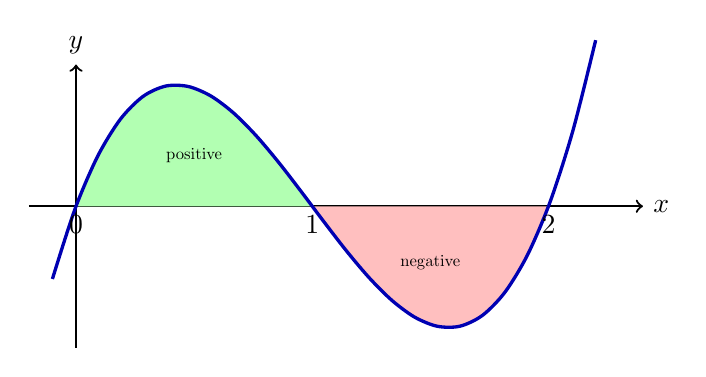
\begin{tikzpicture}[xscale=3,yscale=4]
\draw[->,thick] (-0.2,0)--(2.4,0) node[right] {$x$};
\draw[->,thick] (0,-0.45)--(0,0.45) node[above] {$y$};
\fill[green!30] (0,0)--plot[smooth,domain=0:1] (\x,{\x*(\x-1)*(\x-2)})--(1,0)--cycle;
\fill[red!25] (1,0)--plot[smooth,domain=1:2] (\x,{\x*(\x-1)*(\x-2)})--(2,0)--cycle;
\draw[very thick,blue!70!black] plot[smooth,domain=-0.1:2.2] (\x,{\x*(\x-1)*(\x-2)});
\node[below] at (0,0) {$0$}; \node[below] at (1,0) {$1$}; \node[below] at (2,0) {$2$};
\node[scale=.6] at (0.5,0.16) {positive}; \node[scale=.6] at (1.5,-0.18) {negative};
\end{tikzpicture}
\end{document}